Single crystals show a nicely ordered, clean surface - two properties important for reliable and reproducible experiments. We have chosen silver and copper as bulk crystalline substrates. Both metals form fcc lattices and their surface termination can be fixed by precise cutting along a symmetry plane of choice. For the course of this thesis, experiments are conducted mainly on (111) and (100) terminated surfaces as depicted in \autoref{fig:crystal-termination}.

The lattice constants a at room temperatures for \underline{\textbf{cite!}} Cu(\SI{3,61}{\angstrom}), Ag(\SI{4,09}{\angstrom}) and Au(\SI{4,07}{\angstrom}) are related to the nearest neighbor (NN) distances by multiplication with $\frac{\sqrt{2}a}{2}$. This makes the NN distances $NN: Cu_{111}(\SI{2,55}{\angstrom}), Ag_{111}(\SI{2,89}{\angstrom}) and Au_{111}(\SI{2,88}{\angstrom}$. $\textnormal{2}^{nd}$ NN distance is $a$. When the surface facet is (100), nearest neighbor distances remain the same, only the $\textnormal{2}^{nd}$ NN distance is increased by multiplication with $\sqrt{2}a\cos(\frac{\beta}{2}$ (see \autoref{tab:lattice-constants}).

Lattice constants are related to environment temperatures by their expansion coefficients.
Coefficients of \SI{16,5e-6}{\per \kelvin}(Cu), \SI{18,9e-6}{\per \kelvin}(Ag) and \SI{14,2e-6}{\per \kelvin}(Au) make the substrate lattice shrink by $\approx \SI{0,5}{\percent}$ when it is cooled down from RT to low temperature measurement conditions (\SIrange{5}{7}{\kelvin}) in STM/AFM. This is negligible for bulk materials that are not heated and cooled over large temperature ranges. When an ad layer is adsorbed, different thermal expansion coefficients cause strain in the ad layer. The effect is amplified when metal substrate and ad layer (\textit{h}-BN)
have thermal expansion coefficients with opposite sign (\textcolor{red}{\textbf{Give expansion coefficient and lattice constant for \textit{h}-BN}}).\cite{farwick_zum_hagen_structure_2016}

\begin{table}
\centering \index{Crystal:lattice constants}
\caption{Inter atomic distances for Cu and Ag with respect to different surface termination. $a$ denotes the lattice constant and $\beta= \SI{60}{\deg}$ the angle within the (111) unit cell}
\label{tab:lattice-constants}
  \begin{tabular}{ccccc}
& Lattice constant a [\SI{}{\angstrom}] & Nearest neighbors [\SI{}{\angstrom}] & diagonal [\SI{}{\angstrom}]\\ \hline 
\multicolumn{2}{c}{fcc(100)} & $\frac{\sqrt{2}a}{2}$ & a \\
  Cu	 	& 3.61	& 2.55 | 2.55 & 3.61  \\
  Ag		& 4.09	& 2.89 | 2.89 & 4.09 \\ \hline 
\multicolumn{2}{c}{fcc(111)} & $\frac{\sqrt{2}a}{2} \ <110>$ & $\sqrt{2}a\sin(\frac{\beta}{2})$ | $\sqrt{2}a\cos(\frac{\beta}{2})$\\
Cu 		& 3.61	& 2.55 | 2.55	& 2.55 | 4.42 \\
Ag		& 4.09	& 2.89 | 2.89	& 2.89 | 5.01 \\ \hline
 \end{tabular}
\end{table}

\begin{figure}\centering
	\subfigure[(111)]{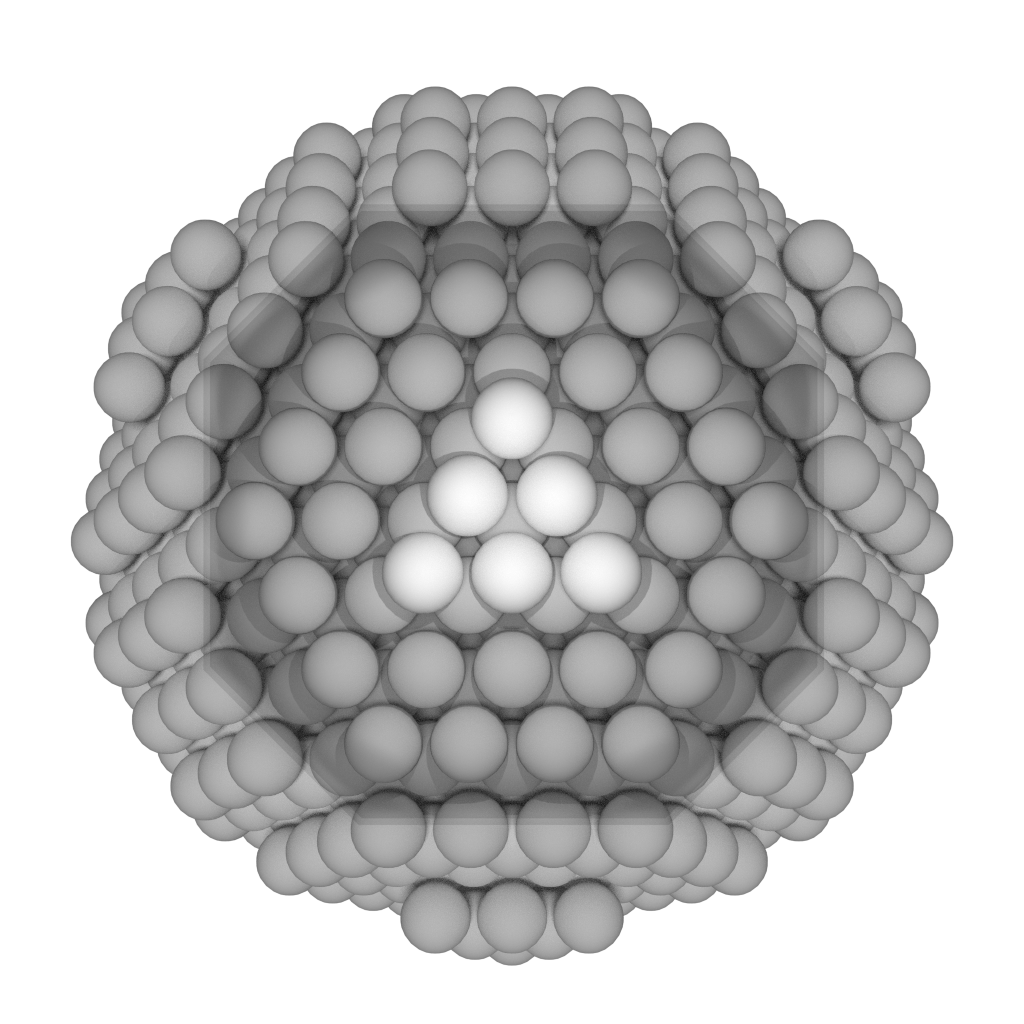
\includegraphics[width=0.3\textwidth]{./images/fcc-111-persp}} \quad
	\subfigure[(100)]{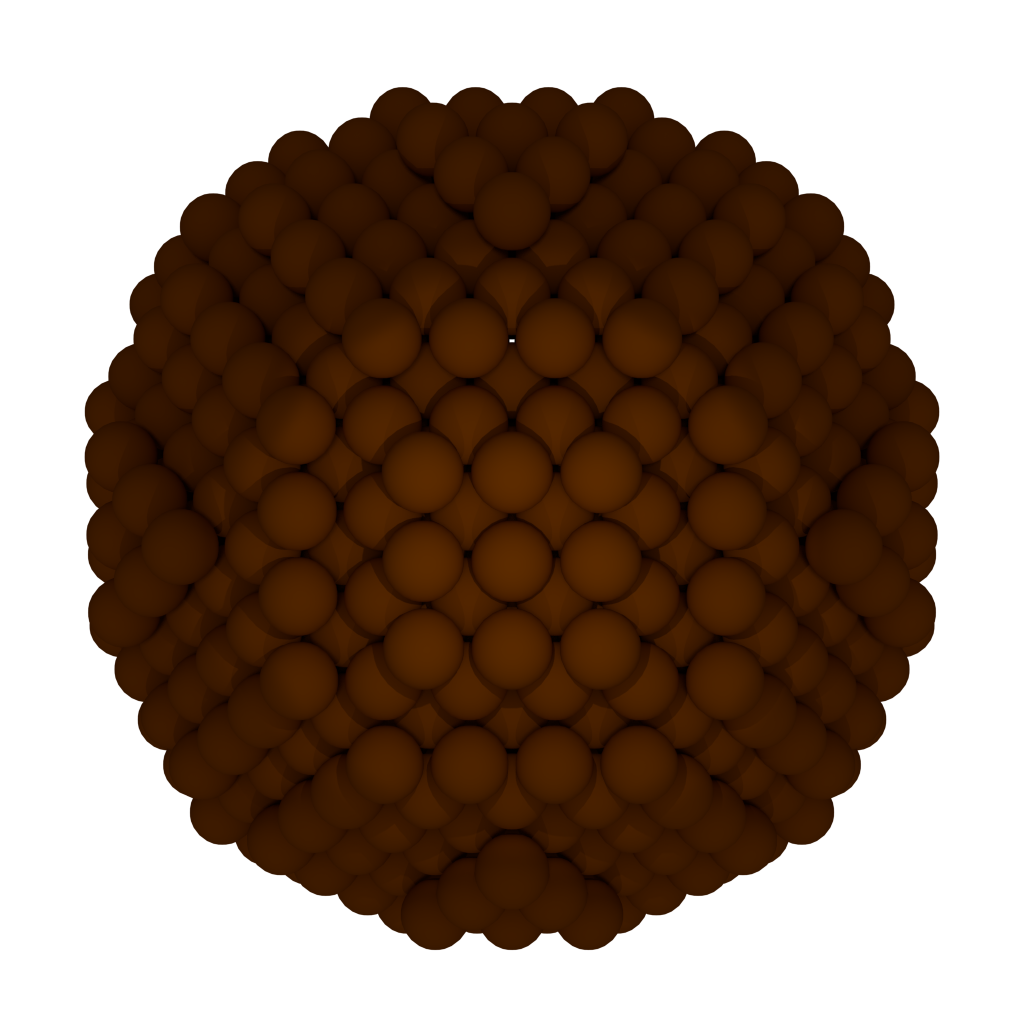
\includegraphics[width=0.3\textwidth]{./images/fcc-100-persp}}
%	\subfigure[(110)]{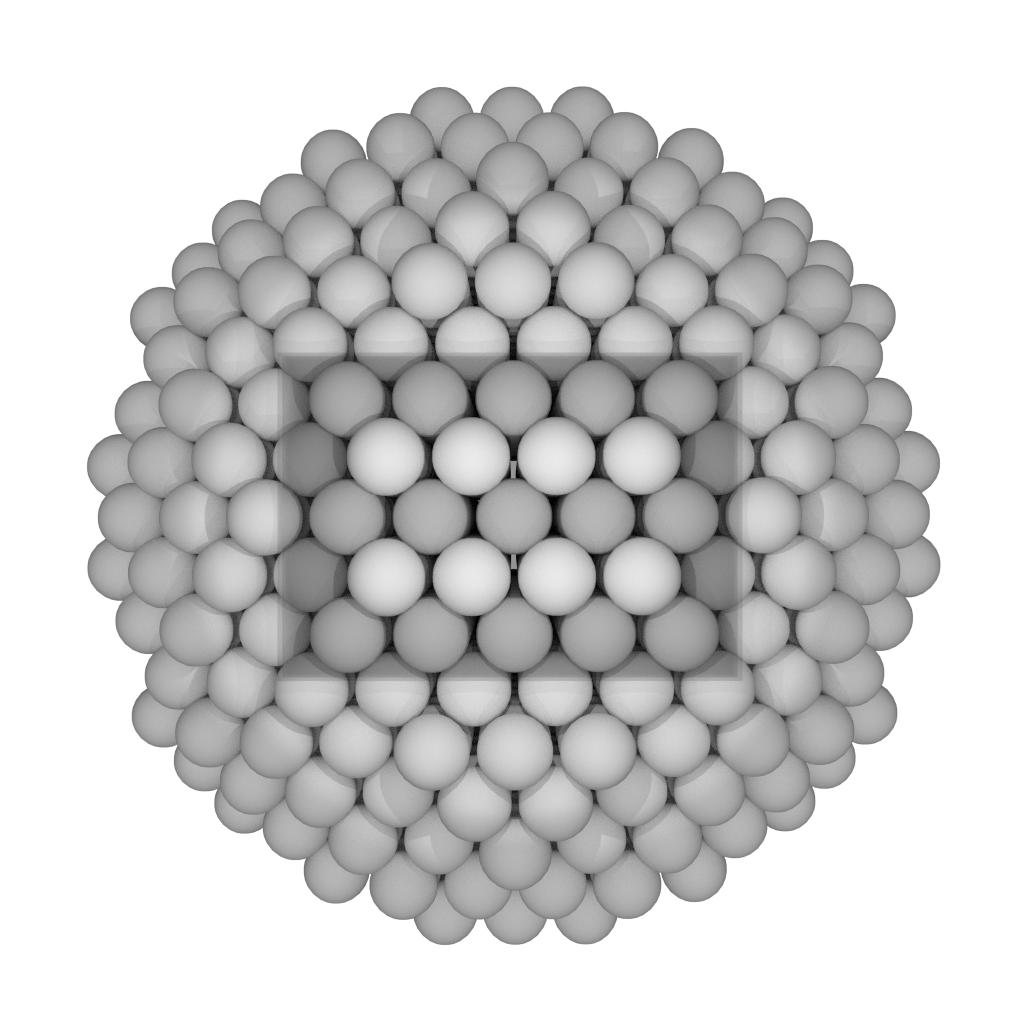
\includegraphics[width=0.3\textwidth]{./images/fcc-110-persp}}
	\caption{Identical crystalline balls with fcc lattice and $\textnormal{[ABC]}_n$ stacking configuration of crystal planes. The surface termination is determined by the direction of the intersecting plane (parallel to the paper plane) relative to the lattice and forms (111) and (100) surfaces.}
	\label{fig:crystal-termination}
\end{figure}

The surface free energy increases from the (111) surface with increasing angle of the (hkl) planes of interest with $$\cos(\phi)=\frac{h+k+l}{\sqrt{3(h^2+k^2+l^2)}}$$ \cite{jian-min_calculation_2004}. Thus, the (111) surface is the one with lowest energy, followed by (110) and (100). For polycrystalline foils it is expected to observe the lowest energy facet more often than the less favorable (110) and (100) facet.

\textcolor{red}{\textbf{Work functions, Surface state, Reactivity - all depend on facet orientation}}

 \subsection{Polycrystalline copper foils}
 
  As was mentioned before, clean, highly ordered surfaces are desirable to perform experiments on. In case a systems order and functionality does not heavily depend on the substrates crystalline properties, single crystals loose most of their unique selling point. Instead of choosing a expensive bulk single crystal, thin polycrystalline copper foils are an alternative. The mass produced foils, although chemically pure, were never meant to be atomically flat and show considerable height variation.

\begin{wrapfigure}{O}{4cm}\centering
	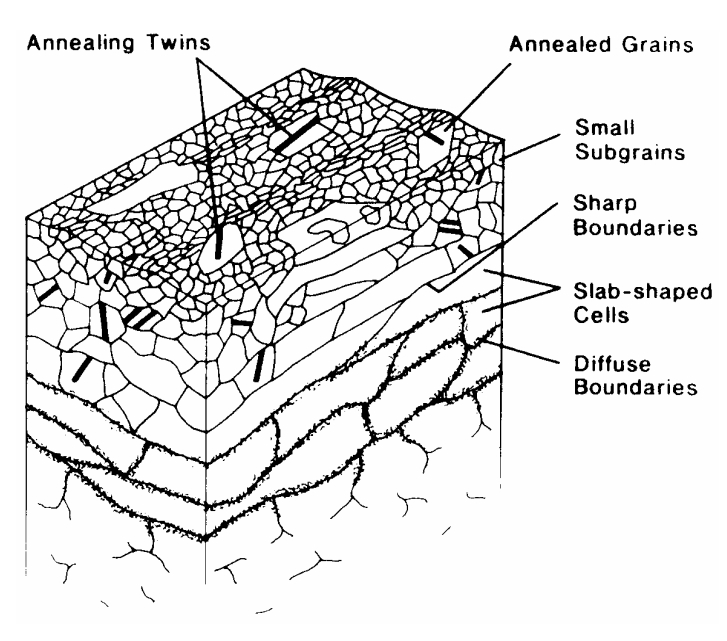
\includegraphics[height=40mm]{./images/grain-structure-copper-foil}
	\caption{Sketched bulk structure of a OFHC copper foil after abrasion with P1200 silicon carbide paper. Adopted from \cite{turley_nature_1981}}
	\label{fig:copper-foil-grains}
\end{wrapfigure}

 A representation of a mechanically polished copper surface can be seen in \autoref{fig:copper-foil-grains}. Here the layered structure is apparent and shows different sizes of grains. Small sub grains constitute the uppermost layers, while deeper lying layers consist of larger grains with grain boundaries becoming more and more diffuse with increasing distance to the surface. 
 
To overcome the limitation of small grain size and heavily corrugated surface, etching of the copper foil is performed as described in \autoref{sec:etching}.